%%%%%%%%%%%%%%%%%%%%%%%%%%%%%%%%%%%%%%%%%%%%%%%%%%%%%%%%%%%%%%%%%%%
%%%%%%%%%%%%%%%%%%%%%%%%%%%%%%%%%%%%%%%%%%%%%%%%%%%%%%%%%%%%%%%%%%%
\begin{frame}{Conclusions}

\vspace{0.1cm}
\begin{itemize}
\item Deep Learning (DL) is a promising alternative for solving geophysical inverse problems.
\vspace{0.3cm}
\item We need efficient DL solvers of PDEs.
\vspace{0.3cm}
\item New challenges arise when solving PDEs using DL: Regularity, Quadrature, and Minimization.
\vspace{0.3cm}
\item Deep-FEM, r-Adaptivity, and Deep-Fourier Residual methods are suitable novel DL solvers for PDEs.
\vspace{0.3cm}
\item {\color{red}{DL solvers for PDEs are at their infancy: we have work ahead....}}
\end{itemize}
%\begin{tikzpicture}
%\node  at (0,0) {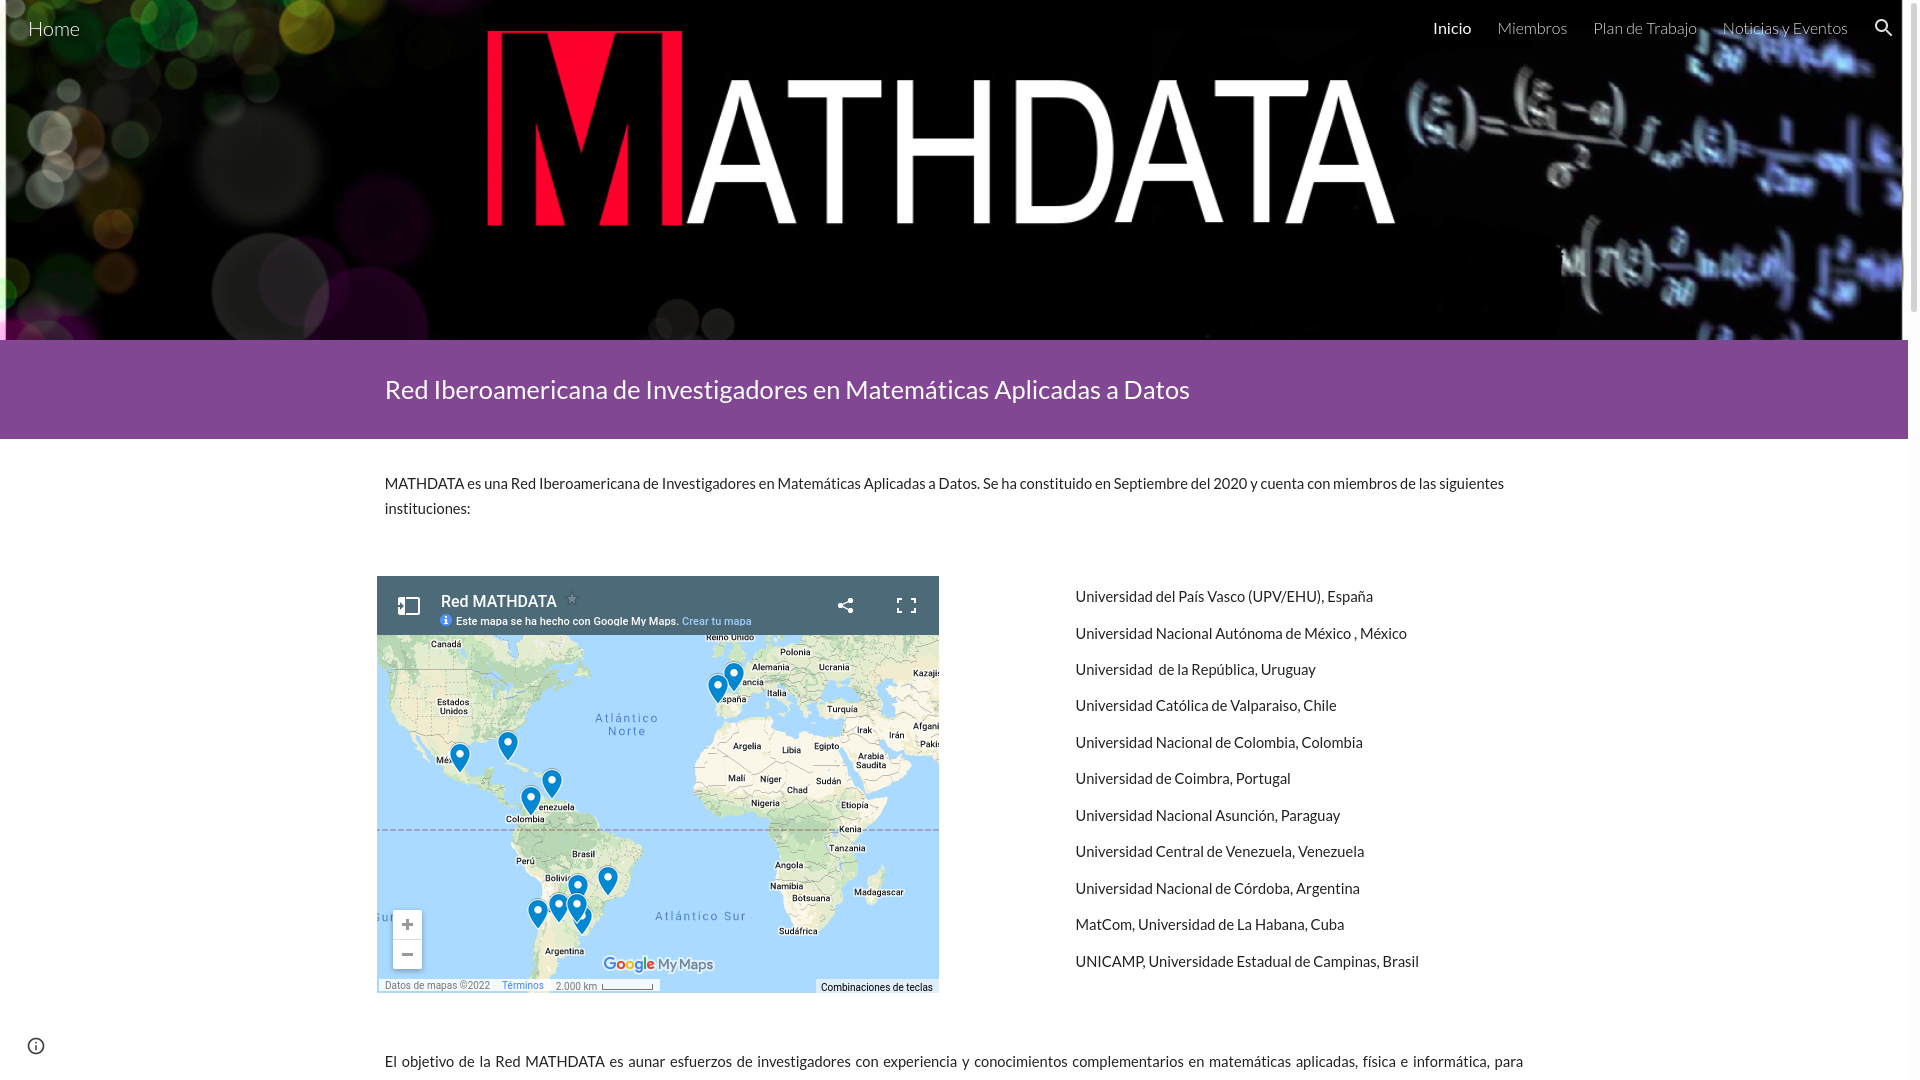
\includegraphics[scale=0.11]{frames/Javi/img/mathdata.png}};
%\node  at (6.5,2) {Red Iberoamericana: Mathdata};
%\node at (7.5,1.3){\href{https://www.mathdata.science/}{https://www.mathdata.science/}};
%
%\node  at (6.5,-2.5) {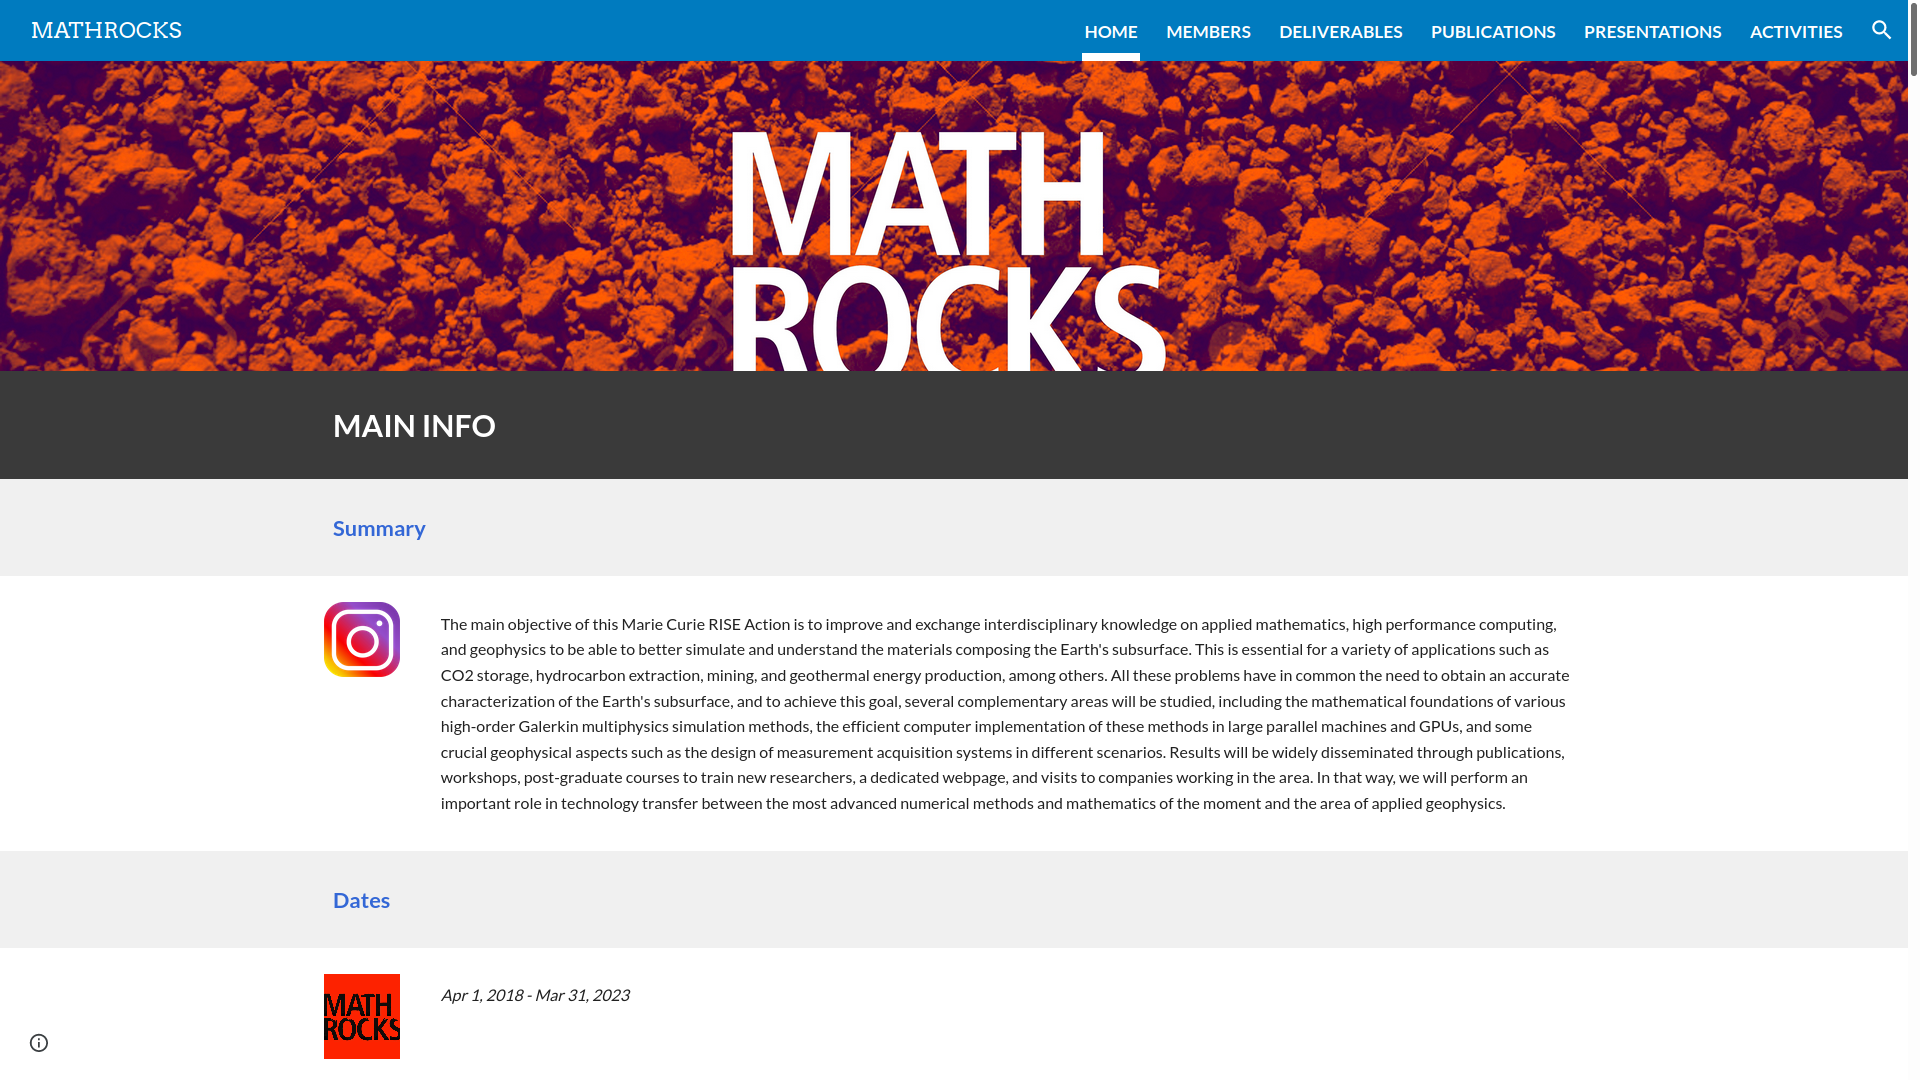
\includegraphics[scale=0.11]{frames/Javi/img/mathrocks.png}};
%\node at (-1,-3.5){International Project: Mathrocks};
%\node at (0,-4.2){\href{https://www.mathrocks.science/}{https://www.mathrocks.science/}};
%
%
%\end{tikzpicture}

\end{frame}
%%%%%%%%%%%%%%%%%%%%%%%%%%%%%%%%%%%%%%%%%%%%%%%%%%%%%%%%%%%%%%%%%%%



